\documentclass[border=5pt]{standalone}

\usepackage{amsmath, amsfonts}
\usepackage{tikz}
\usetikzlibrary{arrows, matrix, calc}

\newcommand{\athir}[2]{\displaystyle H^{#1}(\B G; H^{#2}(\widetilde{M}))}
\newcommand{\zz}{\ensuremath\mathbb{Z}_2}
\newcommand{\B}{\ensuremath\mathrm{B}}


\begin{document}
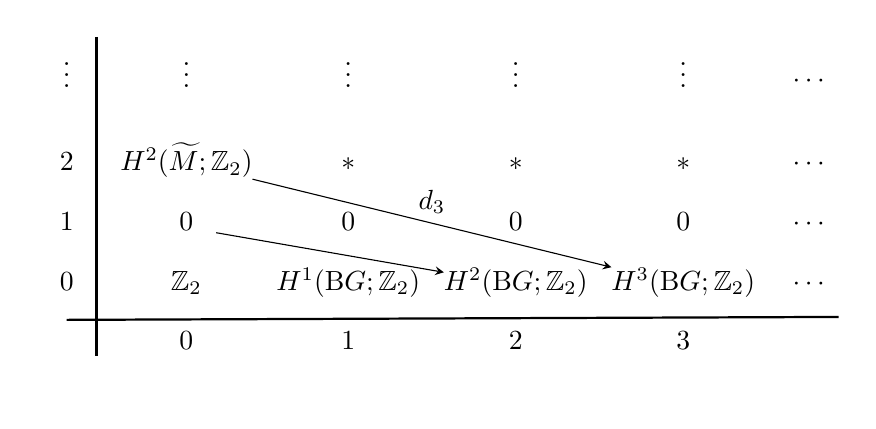
\begin{tikzpicture}
\matrix (m) [matrix of math nodes,
             nodes in empty cells,
             nodes={minimum width=5ex, minimum height=6ex,
                    text depth=1ex,
                    inner sep=0pt, outer sep=0pt,
                    anchor=base},
             column sep=2ex, row sep=2ex]%
{
\vdots  & \vdots       & \vdots       & \vdots & \vdots       & \cdots \\
    [5ex,between origins]
    2 & H^2(\widetilde{M};\zz) & \ast & \ast & \ast & \cdots \\
    [3ex,between origins]
    1   &   0 & 0 & 0 & 0 & \cdots \\
    [3ex,between origins]
    0   &   \zz & H^1(\B G;\zz) & H^2(\B G; \zz) & H^3(\B G; \zz) & \cdots \\
    [3ex,between origins]
        &  0           &  1           & 2 &  3         & \strut \\
};
\draw[-stealth] (m-2-2) -- node[above] {$d_3$} (m-4-5);
\draw[-stealth] (m-3-2) --  (m-4-4);

\draw[thick] (m-1-1.north east) -- (m-5-1.east) ;
\draw[thick] (m-5-1.north) -- ($(m-4-6.east)!0.5!(m-5-6.east)$) ;
\end{tikzpicture}


\end{document}

